%%%%%%%%%%%%%%%%%%%%%%%%%
\section{\label{sec:rhs_smuvt}Unbiased semi-grand canonical (semi-$\mu VT$) ensemble trials}
%%%%%%%%%%%%%%%%%%%%%%%%%

Semi-$\mu VT$ trials have fixed total numbers of particles, but the composition may change \cite{kofke_monte_1988}.
For a trial in which particles of type $i$ may be replaced with particles of type $j$, and vice versa, the probability of a microstate in the semi-$\mu VT$ ensemble is proportional to \cite{kofke_monte_1988}
\begin{equation}
\Pi(N_i,N_j) \diff\mathbf{r}^N \diff\boldsymbol{\omega}^N\propto z_i^{N_i} z_j^{N_j} e^{-\beta U} \diff\mathbf{r}^N\diff\boldsymbol{\omega}^N.
\label{eq:rhs_smuvt_pi}
\end{equation}
Using Eq.~\ref{eq:rhs_smuvt_pi}, the ratio of microstate probabilities of the semi-$\mu VT$ ensemble in Eq.~\ref{eq:detailed_balance} is given by
\begin{equation}
\frac{\Pi_n}{\Pi_o} = z_i^{\Delta N_i}z_j^{\Delta N_j} e^{-\beta\Delta U}.
\label{eq:rhs_sgcmc}
\end{equation}
with the constraint that $\Delta N_i + \Delta N_j = 0$.

%%%%%%%%%%%%%%%%%%%%%%%%%
\subsection{\label{sec:lhs_sgcmc}Changing particle type}
%%%%%%%%%%%%%%%%%%%%%%%%%

The semi-$\mu VT$ ensemble described in Section~\ref{sec:rhs_smuvt} allows particles of one type to change into another, as shown in Fig.~\ref{fig:sgcmc}.
A particle type change trial proceeds as follows.
First, the trial is defined with a number of particle types, $n$ that many change into each other.
Thus, there are $N_m=\sum_i^{mobile} N_i$ changeable particles.
One of those particles is randomly chosen with probability $1/N_m$.
If the type of the chosen particle is given by $i$, then choose a random particle of type $j \neq i$ from among the $n-1$ other particle types.
Then, add a particle of type $j$ with a predetermined interaction site at the same coordinates as a predetermined interaction site in the chosen particle.
Finally, remove the chosen particle, and randomly orient the newly added particle.
The transition probabilities are summarized in Table~\ref{tab:lhs_sgcmc}.

\begin{figure}
\begin{centering}
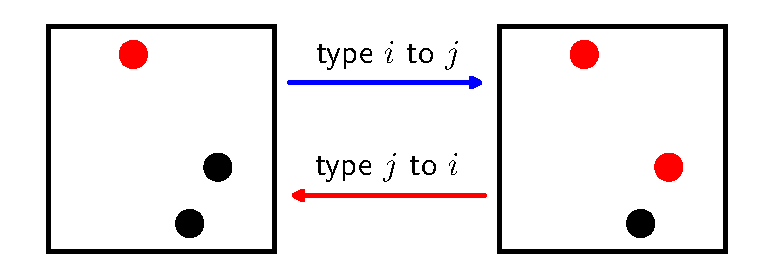
\includegraphics[width=8.5cm]{../figures/sgcmc.pdf}
\caption{
Semi-$\mu VT$ change of a particle of type $i$, shown in red, into a particle of type $j$, shown in black.
The total number of particles remains constant.
}
\label{fig:sgcmc}
\end{centering}
\end{figure}

\begin{table}
\begin{center}
\begin{tabular}{|c|c|}
 \hline
 \thead{Forward} & \thead{$\alpha_{o\rightarrow n}$} \\ [0.5ex]
 \hline
 Choose a particle of any type & $1/N_m$ \\
 \hline
 Choose new particle type $j$ & $1/(n-1)$ \\
 \hline
 Choose orientation & $P_{\omega j}\diff\boldsymbol{\omega}$ \\
 \hline
 \hline\hline
 \thead{Reverse} & \thead{$\alpha_{n\rightarrow o}$} \\ [0.5ex]
 \hline
 Choose particle of any type & $1/N_m$ \\
 \hline
 Choose new particle type $i$ & $1/(n-1)$ \\
 \hline
 Choose orientation & $P_{\omega i}\diff\boldsymbol{\omega}$ \\
 \hline
\end{tabular}
\caption{Particle type change transition probabilities.}
\label{tab:lhs_sgcmc}
\end{center}
\end{table}


Using Table~\ref{tab:lhs_sgcmc} and substituting Eq.~\ref{eq:rhs_sgcmc} into Eq.~\ref{eq:detailed_balance}, the acceptance probability for the $i\rightarrow j$ attempt as the forward transition is
\begin{equation}
\chi = \left(\frac{P_{\omega j}}{P_{\omega i}}\right)\frac{z_j}{z_i}e^{-\beta\Delta U}.
\label{eq:chisgcmc}
\end{equation}
If the particles are isotropic, or rigid and random orientations are chosen, $P_{\omega j}=P_{\omega i}$.
Otherwise, $\frac{P_{\omega j}}{P_{\omega i}}$ is related to the Rosenbluth factors for configuration bias partial regrowth or orientational bias.
Eq.~\ref{eq:chisgcmc} is tested against an $n=2$ component ideal gas mixture in Code Block~\ref{sim:ideal_gas_sgcmc}.

\begin{figure}
\lstinputlisting[
language=Python,
label={sim:ideal_gas_sgcmc},
caption={Semi-$\mu VT$ MC of a two component ideal gas mixture using Python 3, and the statistics module is provided in Section~\ref{sec:block_av}.}
]{../codes/ideal_gas_sgcmc.py}
\end{figure}

%%%%%%%%%%%%%%%%%%%%%%%%%
\subsection{\label{sec:lhs_sgcmc_alt}Changing particle type by choosing a specific type}
%%%%%%%%%%%%%%%%%%%%%%%%%

In the previous Section~\ref{sec:lhs_sgcmc}, particles of multiple types are chosen randomly to attempt a change into another particle type.
Instead of choosing from all particles of any type, an alternative method is to choose one type specifically to change into another.
However, this alternative algorithm changes the acceptance criteria.

An alternative particle type change trial proceeds as follows.
First, a $i \rightarrow j$ or $j \rightarrow i$ trial is randomly chosen with equal probability.
For $i \rightarrow j$, a particle of type $i$ is randomly chosen.
A particle of type $j$ is added to the system with a fixed site in $j$ at the same position as a fixed site in $i$.
Particle $j$ is randomly oriented or regrown about its fixed site.
Particle $i$ is removed from the system.
For $j \rightarrow i$, a particle of type $j$ is randomly chosen.
A particle of type $i$ is added to the system with a fixed site in $i$ at the same position as a fixed site in $j$.
Particle $i$ is randomly oriented or regrown about its fixed site.
Particle $j$ is removed from the system.

For $i \rightarrow j$ as the forward transition, the transition probabilities are summarized in Table~\ref{tab:lhs_sgcmc_alt}, where $N_i$ and $N_j$ are the numbers of each type of particle before the trial is implemented.
Using Table~\ref{sec:lhs_sgcmc_alt} and substituting Eq.~\ref{eq:rhs_sgcmc} into Eq.~\ref{eq:detailed_balance}, the acceptance probability for the $i\rightarrow j$ attempt as the forward transition is
\begin{equation}
\chi = \frac{N_i}{N_j+1}\left(\frac{P_{\omega j}}{P_{\omega i}}\right)\frac{z_j}{z_i}e^{-\beta\Delta U}.
\label{eq:chisgcmc_alt}
\end{equation}

\begin{table}
\begin{center}
\begin{tabular}{|c|c|}
 \hline
 \thead{Forward} & \thead{$\alpha_{o\rightarrow n}$} \\ [0.5ex]
 \hline
 Choose $i \rightarrow j$ & $1/2$ \\
 \hline
 Choose particle of type $i$ & $1/N_i$ \\
 \hline
 Place $j$ on $i$ & $1$ \\
 \hline
 Choose orientation of $j$ & $P_{\omega j}\diff\boldsymbol{\omega}$ \\
 \hline
 \hline\hline
 \thead{Reverse} & \thead{$\alpha_{n\rightarrow o}$} \\ [0.5ex]
 \hline
 Choose $j \rightarrow i$ & $1/2$ \\
 \hline
 Choose particle of type $j$ & $1/(N_j+1)$ \\
 \hline
 Place $i$ on $j$ & $1$ \\
 \hline
 Choose orientation of $i$ & $P_{\omega i}\diff\boldsymbol{\omega}$ \\
 \hline
\end{tabular}
\caption{Alternative particle type change transition probabilities.}
\label{tab:lhs_sgcmc_alt}
\end{center}
\end{table}

The $j\rightarrow i$ trial is the same as Eq.~\ref{eq:chisgcmc_alt} but with $i$ and $j$ indices swapped.
If $i$ and $j$ are rigid molecules and random orientations are chosen (or if isotropic), $P_{\omega i}=P_{\omega j}$.
Otherwise, $\frac{P_{\omega j}}{P_{\omega i}}$ is related to the Rosenbluth factors for configuration bias partial regrowth.
Eq.~\ref{eq:chisgcmc_alt} is tested against an ideal gas mixture in Code Block~\ref{sim:ideal_gas_sgcmc_alt}.

\begin{figure}
\lstinputlisting[
language=Python,
label={sim:ideal_gas_sgcmc_alt},
caption={Alternative algorithm for semi-$\mu VT$ MC of an ideal gas mixture using Python 3, and the statistics module is provided in Section~\ref{sec:block_av}.}
]{../codes/ideal_gas_sgcmc_alt.py}
\end{figure}
